%! TEX root = ../dsa-review.tex

\noindent The constructor for weighted undirected graph takes an edge list with an extra information, namely the weight of the edge.
When building an adjacency list/matrix, a tuple containing the destination vertex and the weight is pushed.

\begin{python}
class Graph:
    # e.g.,: Graph(n = 3, edges = [[0,1,3],[1,2,1],[0,2,6]])
    # creates a graph with 3 nodes indexed 0, 1, 2,
    # with 0 - 1 (weight 3), 0 - 2 (weight 6), 1 - 2 (weight 1)
    def __init__(self, n: int, edges: list[list[int]]):
        self.n = n
        self.edges = edges

        self.adjList = [[] for _ in range(n)]
        for u, v, weight in edges:
            self.adjList[u].append((v, weight))
            self.adjList[v].append((u, weight))

        self.adjMatrix = [[float("inf") for _ in range(n)] for _ in range(n)]
        for i in range(v):
            self.adjMatrix[i][i] = 0
        for u, v, w in edges:
            self.adjMatrix[u][v] = weight
            self.adjMatrix[v][u] = weight
\end{python}

\section{Shortest Path}

\subsection{Initialization and Edge Relaxation for Single-source Shortest-path Algorithms}

\noindent \hrulefill
\begin{algorithmic}[1]
  \Function{Initialize-Single-Source}{$G, s$} \Comment{$G$ is the graph, $s$ is the starting vertex}
    \State $dist \gets$ array size $|V|$
    \State $prev \gets$ array size $|V|$

    \For{$v \in V$}
      \If{$v = s$}
        $dist[v] \gets 0$
      \EndIf
      \If{$v \neq s$}
        $dist[v] \gets \infty$
      \EndIf
      \State $prev[u] \gets \text{nil}$ \Comment{or $-1$}
    \EndFor
    \Return{$dist, prev$}
  \EndFunction
\end{algorithmic}
\noindent \hrulefill

\noindent \hrulefill
\begin{algorithmic}[1]
  \Function{Relax}{$u, v$}
    \State $d \gets dist[u] + weight(u, v)$
    \If{$dist[v] > d$}
      \State $dist[v] = d$
      \State $prev[v] = u$
    \EndIf
  \EndFunction
\end{algorithmic}
\noindent \hrulefill

\noindent Simply put, relaxation is a process of greedily updating the \textproc{dist} value of a vertex $v$ to the shorter of the current \textproc{dist[v]} or newly discovered edge.
These two are easier to understand in action.

\subsection{Bellman-Ford Algorithm}

Bellman-Ford algorithm computes shortest-path by performing relaxation for every edge $|V| - 1$ times (maximum number of edges in a simple path).
Then it attempts to relax each edge once more, and any additional relaxation would indicate the existence of a negative weight cycle (cycle involving an edge with a negative weight; one can travel this over and over to reduce the cost of path, rendering shortest path meaningless).

\noindent \hrulefill
\begin{algorithmic}[1]
  \Function{Bellman-Ford-shortest-path}{$G, V$} \Comment{$G$ is the graph, $V$ is the vertex list}
    \LComment{Initialize-Single-Source: $O(|V|)$}
    \State $dist \gets$ array size $|V|$
    \State $prev \gets$ array size $|V|$

    \For{$v \in V$}
      \If{$v = s$}
        $dist[v] \gets 0$
      \EndIf
      \If{$v \neq s$}
        $dist[v] \gets \infty$
      \EndIf
      \State $prev[u] \gets -1$
    \EndFor
    \item[]
    \LComment{Visiting each edges and relaxing: $O(|V||E|$)}
    \For{$i = 1$ to $|V| - 1$}
      \For{$e \in E$} \Comment{Edge $e$ connects vertex $u$ and $v$}
        \If{$weight[e]$ + $dist[u]$ $<$ $dist[v]$}
          \State $dist[v] = dist[u] + weight[e]$
          \State $prev[v] = u$
        \EndIf
      \EndFor
      \If{If no relaxation happened in the inner loop}
        \LComment{This means that every edges are relaxed to its shortest path}
        \State \Return{true, $dist, prev$}
      \EndIf
    \EndFor
    \item[]
    \LComment{Visiting each edge to check for negative weight cycle: $O(|E|)$}
    \For{$e \in E$} \Comment{Edge $e$ connects vertex $u$ and $v$}
      \If{$weight[e]$ + $dist[u]$ $<$ $dist[v]$}
        \State \Output{Negative weight edge cycle detected}
        \State \Return{false}
      \EndIf
    \EndFor
    \item[]
    \State \Return{true, $dist, prev$}
  \EndFunction
\end{algorithmic}
\noindent \hrulefill

\subsection{Dijkstra's Algorithm}

\noindent Dijkstra is much like BFS< but instead of regular queue, it uses min-heap priority queue to visit a vertex with minimum cost.
The following pseudocode is a textbook implementation of Dijkstra's algorithm, using a min-heap priority queue that supports modifying priorities of an element after they have been enqueued.

\noindent \hrulefill
\begin{algorithmic}[1]
  \Function{Dijkstra}{$G, s$} \Comment{$s$ is the starting vertex}
    \LComment{Initialize-Single-Source: $O(|V|)$}
    \State $\mathrm{dist} \gets$ array size $|V|$
    \State $\mathrm{prev} \gets$ array size $|V|$

    \For{$v \in V$}
      \If{$v = s$}
        $\mathrm{dist}[v] \gets 0$
      \EndIf
      \If{$v \neq s$}
        $\mathrm{dist}[v] \gets \infty$
      \EndIf
      \State $\mathrm{prev}[u] \gets -1$
    \EndFor
  \item[]
    \State $Q \gets$ a min-heap priority queue
    \ForAll{$v \in G.V$}
      \LComment This inserts $(0, s)$ for the starting vertex $s$ and $(\infty, v)$ for every other vertices
      \State \Call{$Q$.enqueue}{$\mathrm{dist}[v], v$}
    \EndFor
  \item[]
    \While{$Q \neq \emptyset$}
    \State $(\textrm{\_}, u) \gets$ \Call{$Q$.dequeue}{}
    \ForAll{$v \in$ \Call{$G$.adjacency list of $u$}{}}
      \LComment{Edge relaxation}
      \State $d \gets \textrm{dist}[u] +$ \Call{$G$.weight}{$(u, v)$}
      \If{$d < \textrm{dist}[v]$}
        \State $\textrm{dist}[v] = d$
        \State $\textrm{prev}[v] = u$
        \State \Call{$Q$.set-priority}{$(d, v)$}
      \EndIf
    \EndFor
    \EndWhile
  \EndFunction
\end{algorithmic}
\noindent \hrulefill

\noindent In real life, you seldom find an implementation of priority queue with \textsc{set-priority} function.
Instead, you can simply insert the new tuple into the queue when relaxing an edge.

\begin{minted}{python}
    def dijkstra(self, v):
        dist = [float("inf")] * self.n
        prev = [-1] * self.n

        dist[v] = 0
        q = [(0, v)]

        while q:
            priority, u = heappop(q)

            for w, weight in self.adjList[u]:
                candidate = dist[u] + weight
                if candidate < dist[w]:
                    dist[w] = candidate
                    prev[w] = u
                    heappush(q, (candidate, w))

        return dist, prev
\end{minted}

\noindent This version might cause duplicate vertices in the queue.
For example, if a vertex $v$ gets relaxed to the distance value of $9$ by a vertex $u$, then it later gets relaxed to $6$ by a vertex $w$, then there will be both $(6, v)$ and $(9, v)$ present in the queue.
It will not cause any problem since by the time $(9, v)$ is dequeued, vertices adjacent to $v$ would have been relaxed by $(6, v)$.

\noindent To optimize this, we can check if the priority we dequeued matches the value in the $\textrm{dist}$ array.

\begin{python}
    def dijkstra(self, v):
        dist = [float("inf")] * self.n
        prev = [-1] * self.n

        dist[v] = 0
        q = [(0, v)]

        while q:
            priority, u = heappop(q)

            if priority == dist[u]:  # or p <= dist[u]
                for w, weight in self.adjList[u]:
                    candidate = dist[u] + weight
                    if candidate < dist[w]:
                        dist[w] = candidate
                        prev[w] = u
                        heappush(q, (candidate, w))

        return dist, prev
\end{python}

\noindent Because we only enqueue when a vertex is relaxed, $p < \textrm{dist}[u]$ would never happen unless there is a negative weight cycle.

\subsection{Floyd-Warshall All Pairs Shortest Path Algorithm}

Dijkstra and Bellman-Ford are examples of "single source" shortest path algorithm, computing shortest path from a given vertex to other nodes.
Floyd-Warshall algorithm is an "all pairs" shortest path algorithm, computing the shortest path between all pairs of vertices.
It uses an adjacency matrix to compute shortest paths in $O(|V|^3)$ time.

\begin{python}
    def floydWarshall(self):
        # Making a copy of adjacency matrix
        dist = [row[:] for row in self.adjMatrix]

        for k in range(self.n):
            for i in range(self.n):
                for j in range(self.n):
                    dist[i][j] = min(dist[i][j], dist[i][k] + dist[k][j])

        return dist
\end{python}

\section{Minimum Spanning Tree}

\begin{itemize}
  \item Minimum: $\sum weight$ is minimum
  \item Spanning: All vertices in the graph are connected
  \item Tree: No cycle
\end{itemize}

\noindent The subset of edges that connects all vertices in the minimum cost.

\subsection{Cycle and Cut Properties}

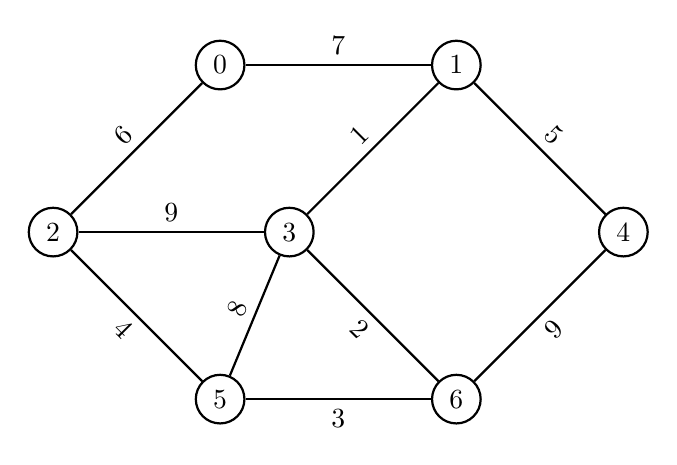
\begin{tikzpicture}[node distance={30mm}, thick, main/.style = {draw, circle}]
  \node[main] (0) {$0$};
  \node[main] (1) [right of=0] {$1$};
  \node[main] (2) [below left of=0] {$2$};
  \node[main] (3) [right of=2] {$3$};
  \node[main] (4) [below right of=1] {$4$};
  \node[main] (5) [below right of=2] {$5$};
  \node[main] (6) [right of=5] {$6$};
  % \draw[->] (1) -- (2);
  \draw[-] (0) -- node[midway, above]{7} (1);
  \draw[-] (0) -- node[midway, above, sloped]{6} (2);
  \draw[-] (1) -- node[midway, above, sloped]{5} (4);
  \draw[-] (1) -- node[midway, above, sloped]{1} (3);
  \draw[-] (2) -- node[midway, above]{9} (3);
  \draw[-] (2) -- node[midway, below, sloped]{4} (5);
  \draw[-] (3) -- node[midway, above, sloped]{8} (5);
  \draw[-] (3) -- node[midway, below, sloped]{2} (6);
  \draw[-] (4) -- node[midway, below, sloped]{9} (6);
  \draw[-] (5) -- node[midway, below]{3} (6);
\end{tikzpicture}

There are two fundamental properties of MST:

\begin{enumerate}
  \item \textit{Cycle Property}: For any cycle $C$ in the graph, if the weight of an edge $e \in C$ is higher than any of individual weights of all other edges in $C$, then its edge cannot belong in the MST.\\
    In the example above, $(6, 4)$ in the cycle $2-0-1-4-6-5$ and $(2, 5)$ in the cycle $2-3-5$ cannot be in the MST.
  \item \textit{Cut Property}: For any \textit{cut} (subdivision of graph with disjoint) $C$ in the graph, if the weight of an edge $e$ in the cut-set of $C$ is strictly smaller than the weights of all other edges of the cut-set of $C$, then this edge belongs to all MST of the graph.\\
    If we remove $(0,1)$, $(2,3)$, $(2,5)$, then graph separates into $(0,1)$ and rest of the vertices. Thus, the lowest cost edge $(2, 5)$ must be in the MST.
\end{enumerate}

\subsection{Prim's Algorithm}

\noindent Prim's algorithm is essentially Dijkstra but for finding MST.

\begin{minted}{python}
    def primMST(self, s, visited):
        dist = [float("inf")] * self.n
        prev = [-1] * self.n

        dist[s] = 0
        q = [(0, s)]

        cost = 0
        mstEdges = []

        while q:
            priority, u = heappop(q)

            # Ensure that the dequed vertex has not been relaxed yet.
            # For the algorithm with implementation without set_priority method
            # See Dijkstra section for more information.
            if priority == dist[u]:
                # update the MST information
                visited[u] = True
                cost += priority
                if prev[u] != -1:
                    mstEdges.append((prev[u], u, priority))

                for v, weight in self.adjList[u]:
                    if not visited[v]:
                        if weight < dist[v]:
                            prev[v] = u
                            dist[v] = weight
                            heappush(q, (weight, v))

        return cost, mstEdges
\end{minted}

\noindent Running the algorithm on the graph in the section 8.2.1, we get the following MST.

\begin{verbatim}
    g = Graph(7, [
        [0, 1, 7],
        [0, 2, 6],
        [1, 4, 5],
        [1, 3, 1],
        [2, 3, 9],
        [2, 5, 4],
        [3, 5, 8],
        [3, 6, 2],
        [4, 6, 9],
        [5, 6, 3]
    ])
    visited = [False] * g.n
    print(g.primMST(0, visited))
    ...
    (21, [(0, 2, 6), (2, 5, 4), (5, 6, 3), (6, 3, 2), (3, 1, 1), (1, 4, 5)])
\end{verbatim}

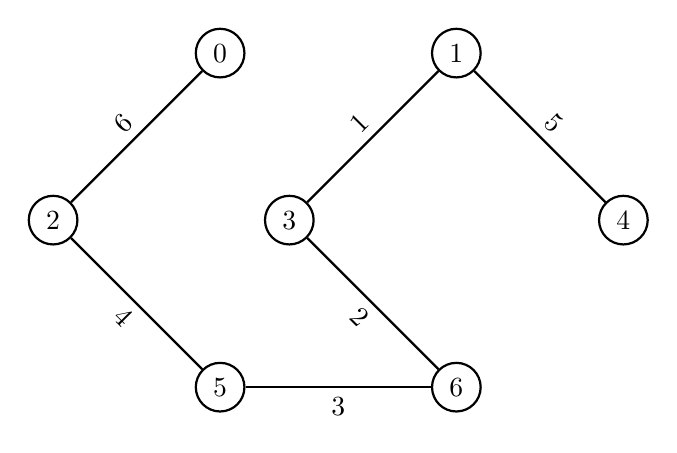
\begin{tikzpicture}[node distance={30mm}, thick, main/.style = {draw, circle}]
  \node[main] (0) {$0$};
  \node[main] (1) [right of=0] {$1$};
  \node[main] (2) [below left of=0] {$2$};
  \node[main] (3) [right of=2] {$3$};
  \node[main] (4) [below right of=1] {$4$};
  \node[main] (5) [below right of=2] {$5$};
  \node[main] (6) [right of=5] {$6$};

  \draw[-] (0) -- node[midway, above, sloped]{6} (2);
  \draw[-] (1) -- node[midway, above, sloped]{1} (3);
  \draw[-] (1) -- node[midway, above, sloped]{5} (4);
  \draw[-] (2) -- node[midway, below, sloped]{4} (5);
  \draw[-] (3) -- node[midway, below, sloped]{2} (6);
  \draw[-] (5) -- node[midway, below]{3} (6);
\end{tikzpicture}


\noindent The Prim's MST algorithm runs in $O(|E| \log (|V|))$.

\noindent The algorithm assumes that the graph is fully connected, so the starting node \textsc{s} can be any node.
However, if the graph is disconnected, you need to run the algorithm on every vertices.

\begin{minted}{python}
    def primAllVertices(self):
        cost = 0
        mstEdges = []
        visited = [False] * self.n
        for v in range(self.n):
            if not visited[v]:
                localCost, localMstEdges = self.primMST(v, visited)
                cost += localCost
                mstEdges.extend(localMstEdges)

        return cost, mstEdges
\end{minted}

\subsection{Union-Find}

Union-Find, or disjoin-set data structure, store sets in terms of their relations to common elements.

\begin{minted}{python}
class UnionFind:
    def __init__(self, n):
        # Initially, each node is parent to itself
        self.parent = list(range(n))

    def findBasic(self, p):
        if self.parent[p] == p:
            return p
        return self.findBasic(self.parent[p])

    def unionBasic(self, p, q):
        rootP = self.find(p)
        rootQ = self.find(q)
        self.parent[rootP] = rootQ
\end{minted}

\noindent The data structure assigns the root/representative of each disjoint set to distinguish each set.

\begin{itemize}
  \item In the beginning, each element is a separate set.
    \begin{center}
      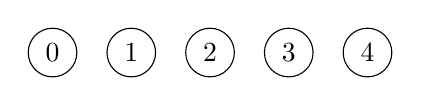
\begin{tikzpicture}[main/.style = {draw, circle}]
        \node[main] (0) {$0$};
        \node[main] (1) [right of=0] {$1$};
        \node[main] (2) [right of=1] {$2$};
        \node[main] (3) [right of=2] {$3$};
        \node[main] (4) [right of=3] {$4$};
      \end{tikzpicture}
    \end{center}
  \item \textsc{Union(1, 0)}: the root of each element is themselves, so $0$ becomes the parent of $1$
    \begin{center}
      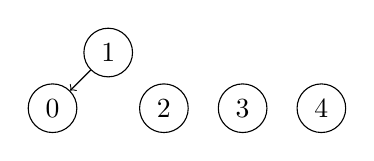
\begin{tikzpicture}[main/.style = {draw, circle}]
        \node[main] (0) {$0$};
        \node[main] (1) [above right of=0] {$1$};
        \node[main] (2) [below right of=1] {$2$};
        \node[main] (3) [right of=2] {$3$};
        \node[main] (4) [right of=3] {$4$};
        %
        \draw[<-] (0) -- (1);
      \end{tikzpicture}
    \end{center}
  \item \textsc{Union(2, 3)}
    \begin{center}
      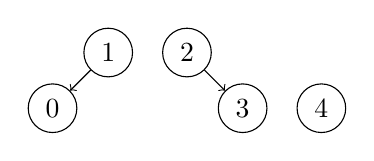
\begin{tikzpicture}[main/.style = {draw, circle}]
        \node[main] (0) {$0$};
        \node[main] (1) [above right of=0] {$1$};
        \node[main] (2) [right of=1] {$2$};
        \node[main] (3) [below right of=2] {$3$};
        \node[main] (4) [right of=3] {$4$};
        %
        \draw[<-] (0) -- (1);
        \draw[->] (2) -- (3);
      \end{tikzpicture}
    \end{center}
  \item \textsc{Union(2, 1)}: the root of $2$ is $3$, the root of $1$ is $0$, so $0$ becomes the parent of $3$
    \begin{center}
      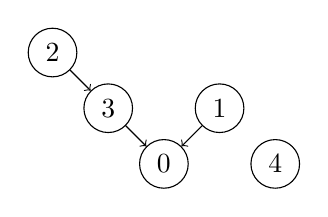
\begin{tikzpicture}[main/.style = {draw, circle}]
        \node[main] (0) {$0$};
        \node[main] (1) [above right of=0] {$1$};
        \node[main] (3) [above left of=0] {$3$};
        \node[main] (2) [above left of=3] {$2$};
        \node[main] (4) [below right of=1] {$4$};
        %
        \draw[<-] (0) -- (1);
        \draw[->] (2) -- (3);
        \draw[->] (3) -- (0);
      \end{tikzpicture}
    \end{center}
  \item \textsc{Union(0, 4)}
    \begin{center}
      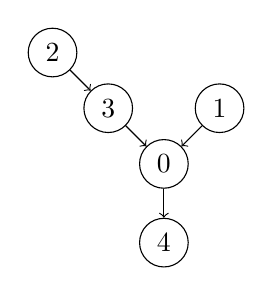
\begin{tikzpicture}[main/.style = {draw, circle}]
        \node[main] (0) {$0$};
        \node[main] (1) [above right of=0] {$1$};
        \node[main] (3) [above left of=0] {$3$};
        \node[main] (2) [above left of=3] {$2$};
        \node[main] (4) [below of=0] {$4$};
        %
        \draw[<-] (0) -- (1);
        \draw[->] (2) -- (3);
        \draw[->] (3) -- (0);
        \draw[->] (0) -- (4);
      \end{tikzpicture}
    \end{center}
\end{itemize}

There are two ways to optimize Union-Find data structure.

\begin{enumerate}
  \item Path Compression (improving \textsc{find})
  \item Union by rank or by size (improving \textsc{union})
\end{enumerate}

\subsubsection{Path Compression}

\begin{minted}{python}
    def findPathCompression(self, p):
        if self.parent[p] != p:
            # path compression
            self.parent[p] = self.findPathCompression(self.parent[p])
        return self.parent[p]
\end{minted}

\noindent Currently, when \textsc{find} is called on $2$, it has to travel multiple elements to get to its root, $4$.
Path compression optimizes the process by "flattening" the tree during the find process.

\noindent After \textsc{find(2)}, the tree becomes:

\begin{center}
  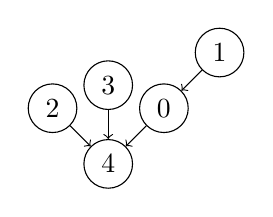
\begin{tikzpicture}[main/.style = {draw, circle}]
    \node[main] (4) {$4$};
    \node[main] (0) [above right of=4]{$0$};
    \node[main] (1) [above right of=0] {$1$};
    \node[main] (3) [above of=4] {$3$};
    \node[main] (2) [above left of=4] {$2$};
      %
    \draw[<-] (0) -- (1);
    \draw[->] (0) -- (4);
    \draw[->] (2) -- (4);
    \draw[->] (3) -- (4);
  \end{tikzpicture}
\end{center}

\subsubsection{Union by Rank}

Union by rank chooses the most efficient node to be the parent of based on the rank (height of the tree if path compression was not used) of the root nodes.

\begin{minted}{python}
class UnionFind:
    def __init__(self, n):
        # Initially, each node is parent to itself
        self.parent = list(range(n))
        self.rank = [0] * n

    def unionByRank(self, p, q):
        rootP = self.find(p)
        rootQ = self.find(q)
        if rootP == rootQ:
            return

        if self.rank[rootP] < self.rank[rootQ]:
            self.parent[rootP] = rootQ
        elif self.rank[rootP] > self.rank[rootQ]:
            self.parent[rootQ] = rootP
        else:
            # you can switch P and Q if you wish
            self.parent[rootP] = rootQ
            self.rank[rootQ] += 1
\end{minted}

\begin{itemize}
  \item In the beginning, each element is a separate set with rank 0
    \begin{center}
      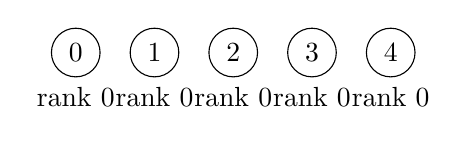
\begin{tikzpicture}[main/.style = {draw, circle}]
        \node[main, label=below:{rank 0}] (0) {$0$};
        \node[main, label=below:{rank 0}] (1) [right of=0] {$1$};
        \node[main, label=below:{rank 0}] (2) [right of=1] {$2$};
        \node[main, label=below:{rank 0}] (3) [right of=2] {$3$};
        \node[main, label=below:{rank 0}] (4) [right of=3] {$4$};
      \end{tikzpicture}
    \end{center}
  \item \textsc{Union(1, 0)}: the root of each element is themselves with equal ranks, we choose $0$ to be the root of $1$ and increase the rank of $0$
    \begin{center}
      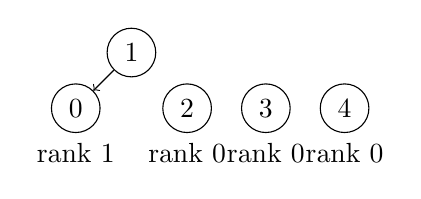
\begin{tikzpicture}[main/.style = {draw, circle}]
        \node[main, label=below:{rank 1}] (0) {$0$};
        \node[main] (1) [above right of=0] {$1$};
        \node[main, label=below:{rank 0}] (2) [below right of=1] {$2$};
        \node[main, label=below:{rank 0}] (3) [right of=2] {$3$};
        \node[main, label=below:{rank 0}] (4) [right of=3] {$4$};
        %
        \draw[<-] (0) -- (1);
      \end{tikzpicture}
    \end{center}
  \item \textsc{Union(2, 3)}
    \begin{center}
      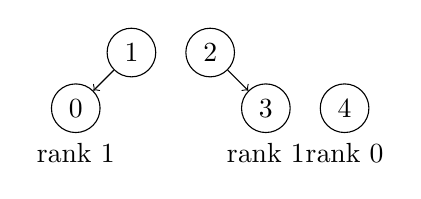
\begin{tikzpicture}[main/.style = {draw, circle}]
        \node[main, label=below:{rank 1}] (0) {$0$};
        \node[main] (1) [above right of=0] {$1$};
        \node[main] (2) [right of=1] {$2$};
        \node[main, label=below:{rank 1}] (3) [below right of=2] {$3$};
        \node[main, label=below:{rank 0}] (4) [right of=3] {$4$};
        %
        \draw[<-] (0) -- (1);
        \draw[->] (2) -- (3);
      \end{tikzpicture}
    \end{center}
  \item \textsc{Union(2, 1)}: \textsc{find(2)} $= 3$ and \textsc{find(1)} $= 0$. Since they are equal in rank, we arbitrarily choose $0$ to be the parent of $3$
    \begin{center}
      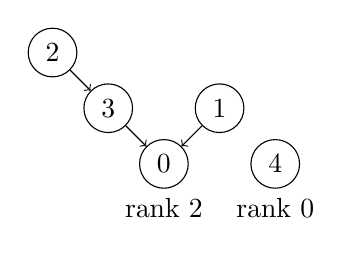
\begin{tikzpicture}[main/.style = {draw, circle}]
        \node[main, label=below:{rank 2}] (0) {$0$};
        \node[main] (1) [above right of=0] {$1$};
        \node[main] (3) [above left of=0] {$3$};
        \node[main] (2) [above left of=3] {$2$};
        \node[main, label=below:{rank 0}] (4) [below right of=1] {$4$};
        %
        \draw[<-] (0) -- (1);
        \draw[->] (2) -- (3);
        \draw[->] (3) -- (0);
      \end{tikzpicture}
    \end{center}
  \item \textsc{Union(0, 4)}: Since $4$ has lower rank than $0$ (the result of \textsc{find(0)}), $0$ becomes the parent of $4$.
    \begin{center}
      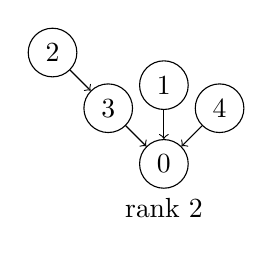
\begin{tikzpicture}[main/.style = {draw, circle}]
        \node[main, label=below:{rank 2}] (0) {$0$};
        \node[main] (1) [above of=0] {$1$};
        \node[main] (3) [above left of=0] {$3$};
        \node[main] (2) [above left of=3] {$2$};
        \node[main] (4) [above right of=0] {$4$};
        %
        \draw[<-] (0) -- (1);
        \draw[->] (2) -- (3);
        \draw[->] (3) -- (0);
        \draw[->] (4) -- (0);
      \end{tikzpicture}
    \end{center}
\end{itemize}

\subsubsection{Union by Size}

I am too lazy to cover it, but here is the Python implementation.
It is essentially union by rank, but it compares the sizes of the trees instead of their heights.

\begin{minted}{python}
class UnionFind:
    def __init__(self, n):
        # Initially, each node is parent to itself
        self.parent = list(range(n))
        self.size = [1] * n


    def unionBySize(self, p, q):
        rootP = self.find(p)
        rootQ = self.find(q)
        if rootP == rootQ:
            return
        if self.size[rootP] < self.size[rootQ]:
            self.parent[rootP] = rootQ
            self.size[rootQ] += self.size[rootP]
        else:
            self.parent[rootQ] = rootP
            self.size[rootP] += self.size[rootQ]
\end{minted}

\subsection{Krustal MST Algorithm}

